\subsection{Wechselstrom-Schalter/Steller}
\subsubsection{Wechselstrom-Schalter}
\begin{minipage}{\linewidth}
    Wegen dem Polaritätswechel besteh der Wechselstromschalter aus zwei antiparallelen Thyristoren, welche die Stromhalbschwingung abwechselnd ausführen.
\end{minipage}

\begin{minipage}{0.3\linewidth}
    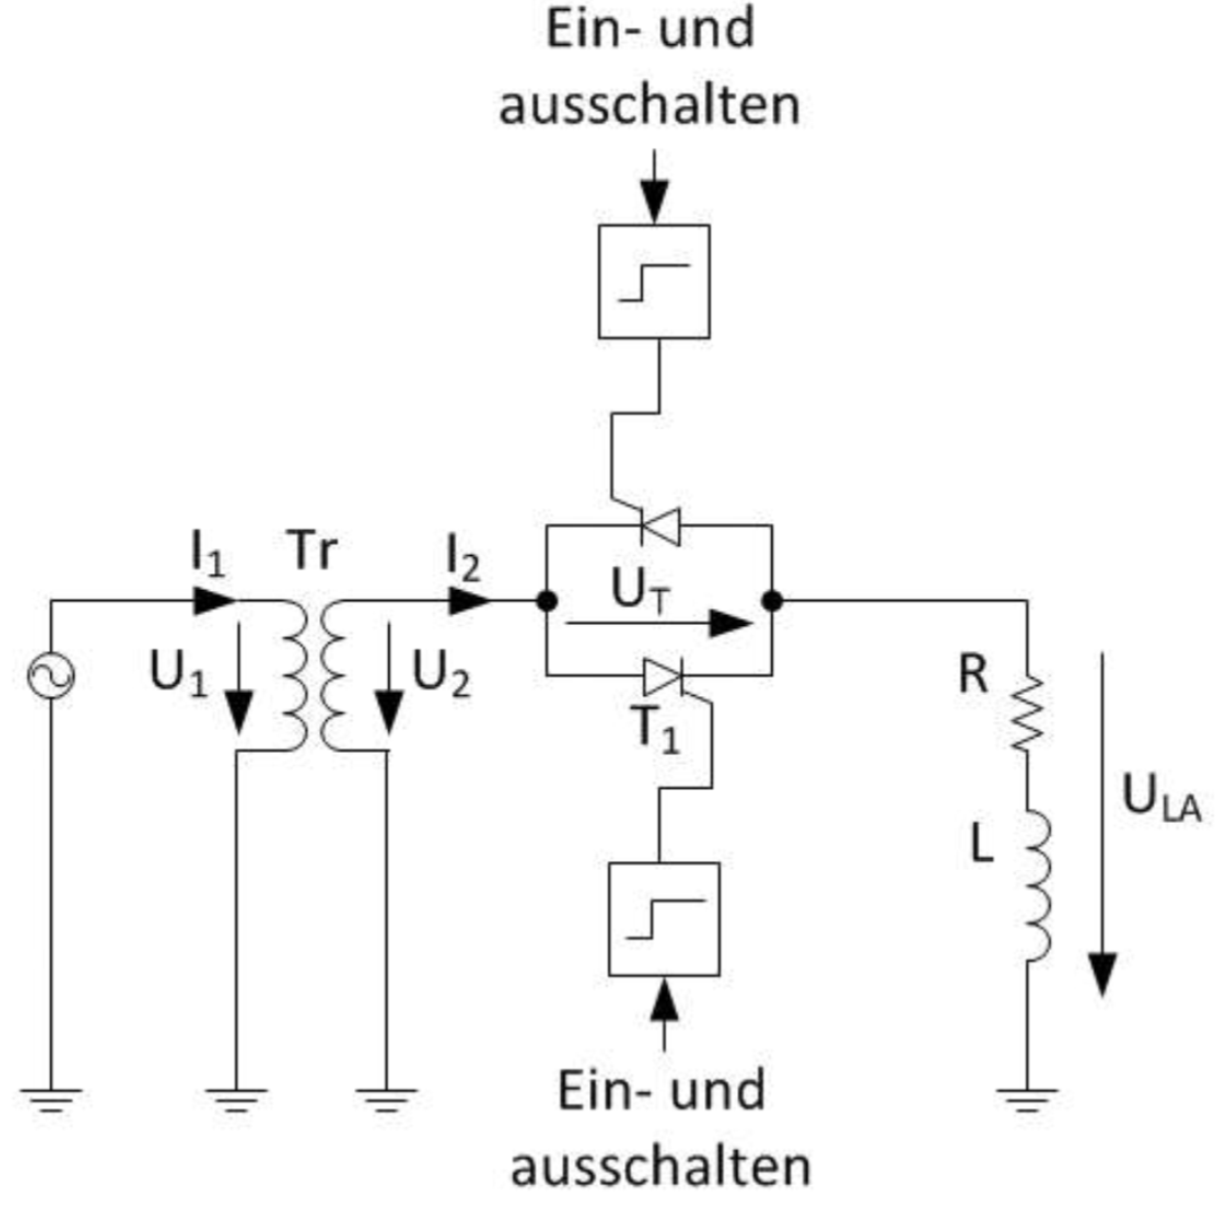
\includegraphics[width=\linewidth]{images/SchemaWSSchalter}
\end{minipage}
\begin{minipage}{0.3\linewidth}
    \textbf{Lasttyp: R}\newline
    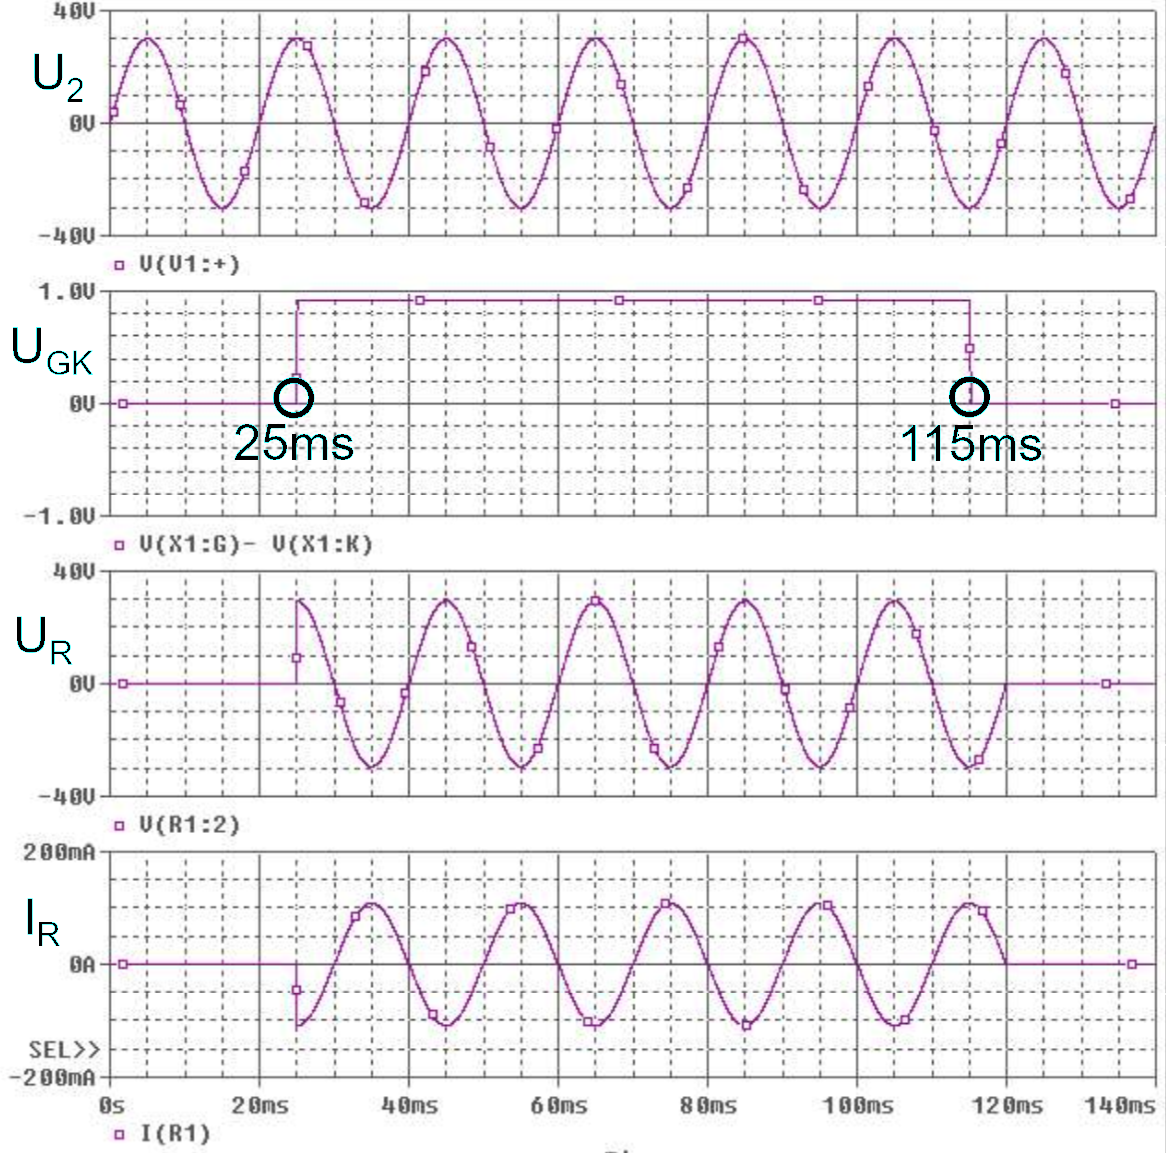
\includegraphics[width=\linewidth]{images/KLWSSchalter}
\end{minipage}
\begin{minipage}{0.3\linewidth}
    \textbf{Lasttyp: R + L}\newline
    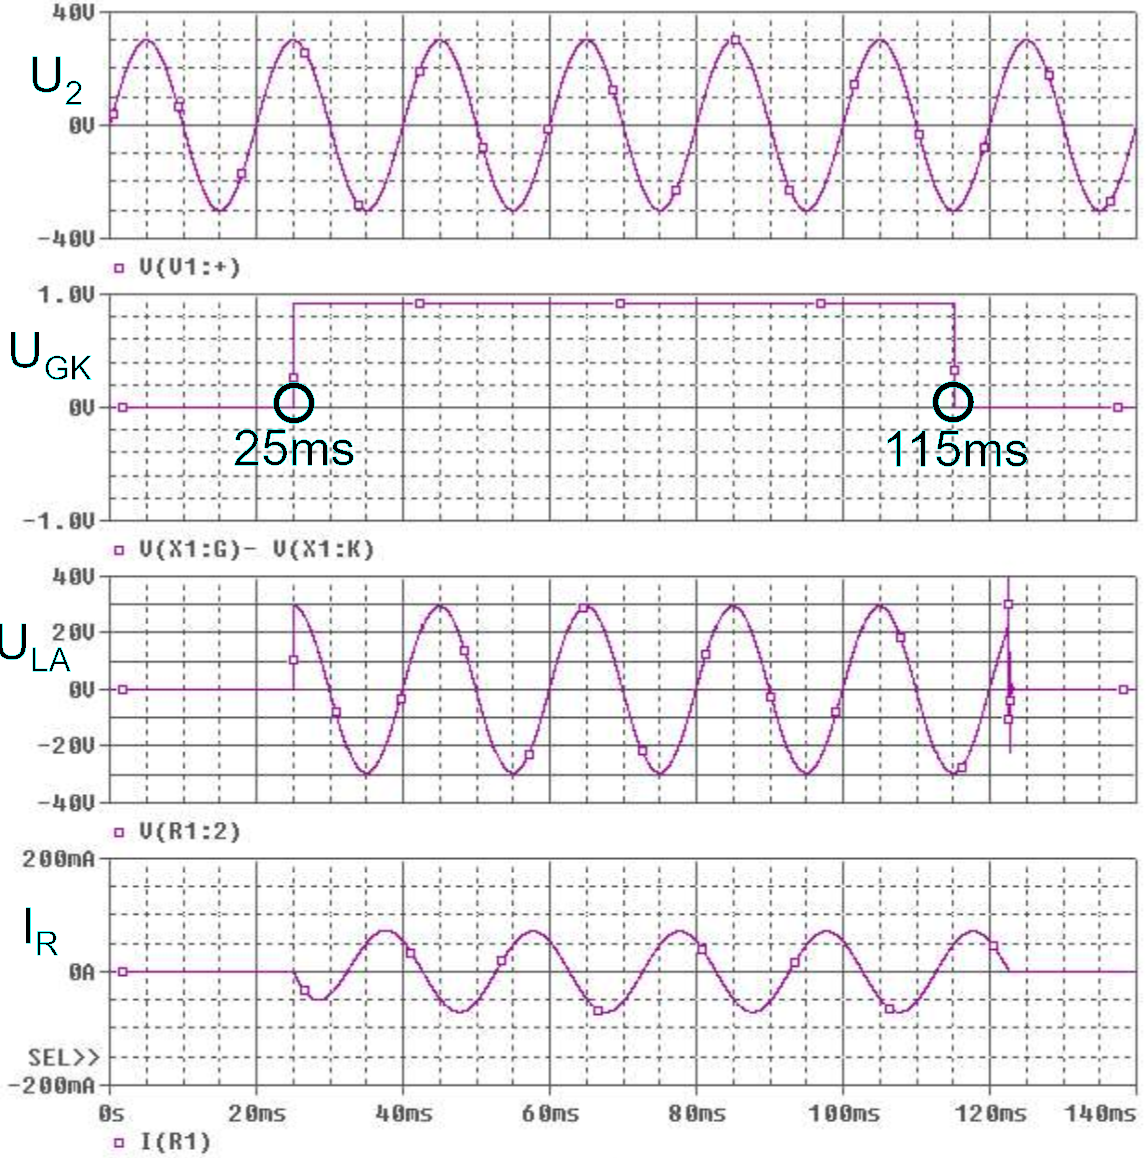
\includegraphics[width=\linewidth]{images/KLWSSchalter2}
\end{minipage}

\subsubsection{Wechselstrom-Steller}
\begin{minipage}{0.5\linewidth}
    Im vergleich mit den Wechselstrom-Schalter, welche eimaligs Ein- oder Ausschalten von Wechselstromkreisen ermöglichen, erlaubt der Wechselstrom-Steller in jeder Halbperiode wiederholtes Einschalten, wobei der Strom vom Zündzeitpunkt bis zm Nulldurchgang fliesst.
\end{minipage}
\begin{minipage}{0.5\linewidth}
    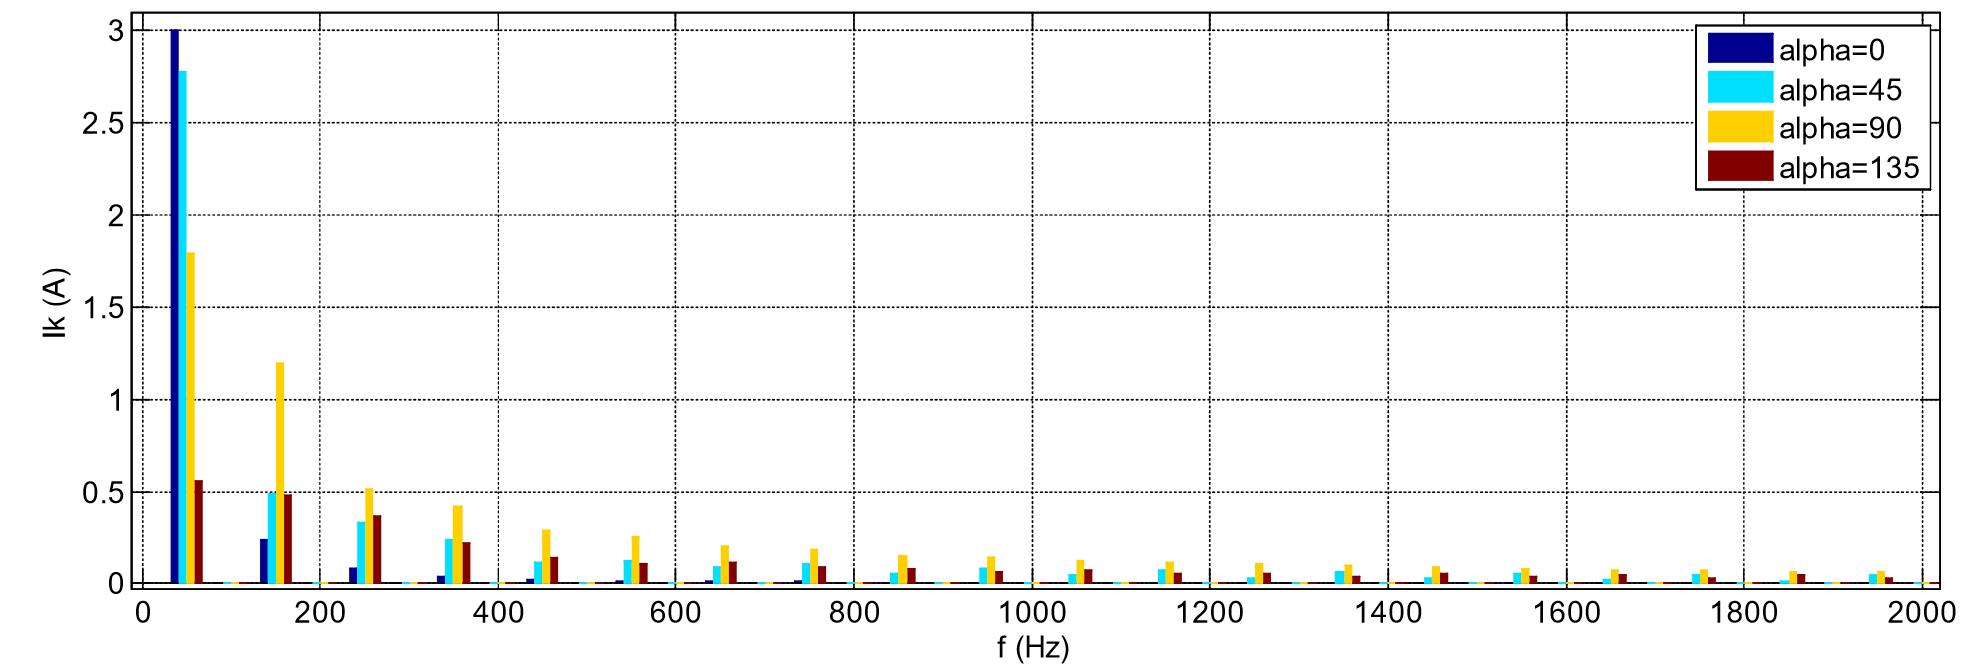
\includegraphics[width=\linewidth]{images/OWWSSteller}
\end{minipage}

\begin{minipage}{0.3\linewidth}
    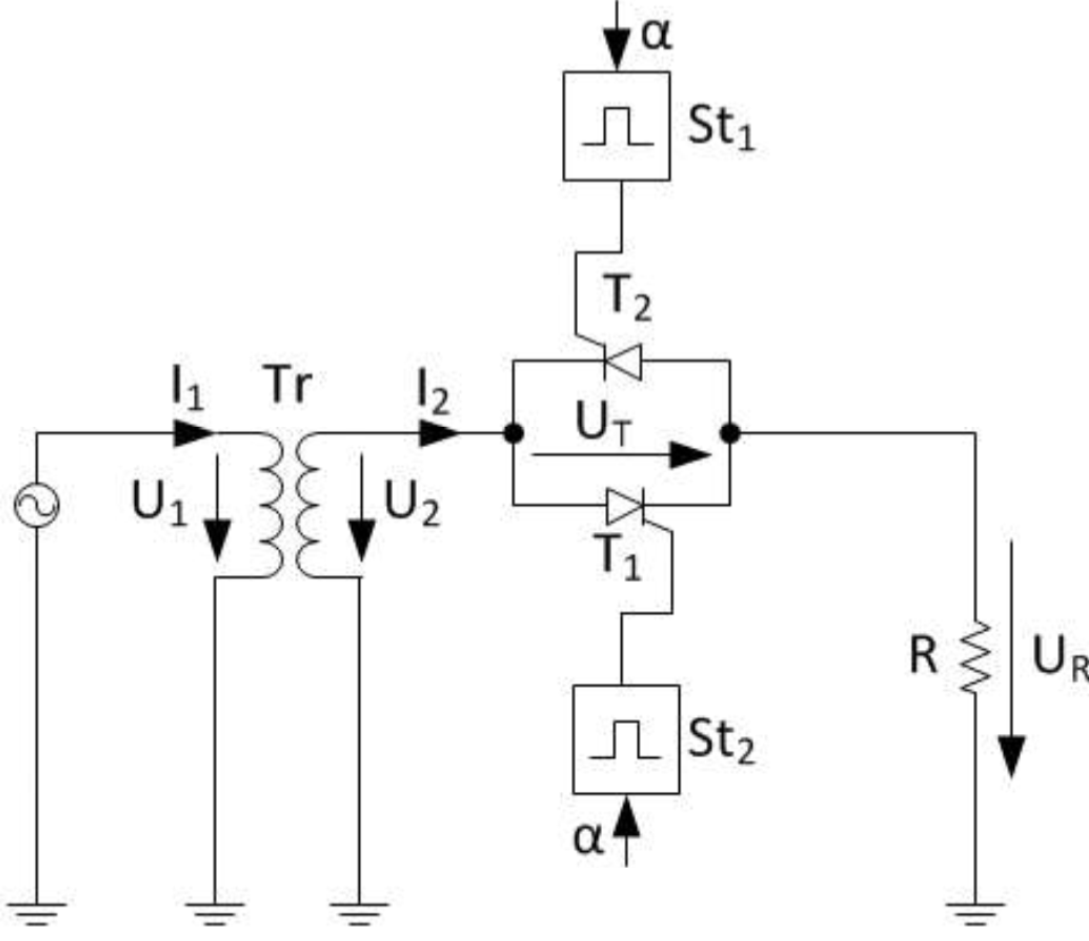
\includegraphics[width=\linewidth]{images/SchemaWSSteller}
\end{minipage}
\begin{minipage}{0.3\linewidth}
    \textbf{Lasttyp: R}\newline
    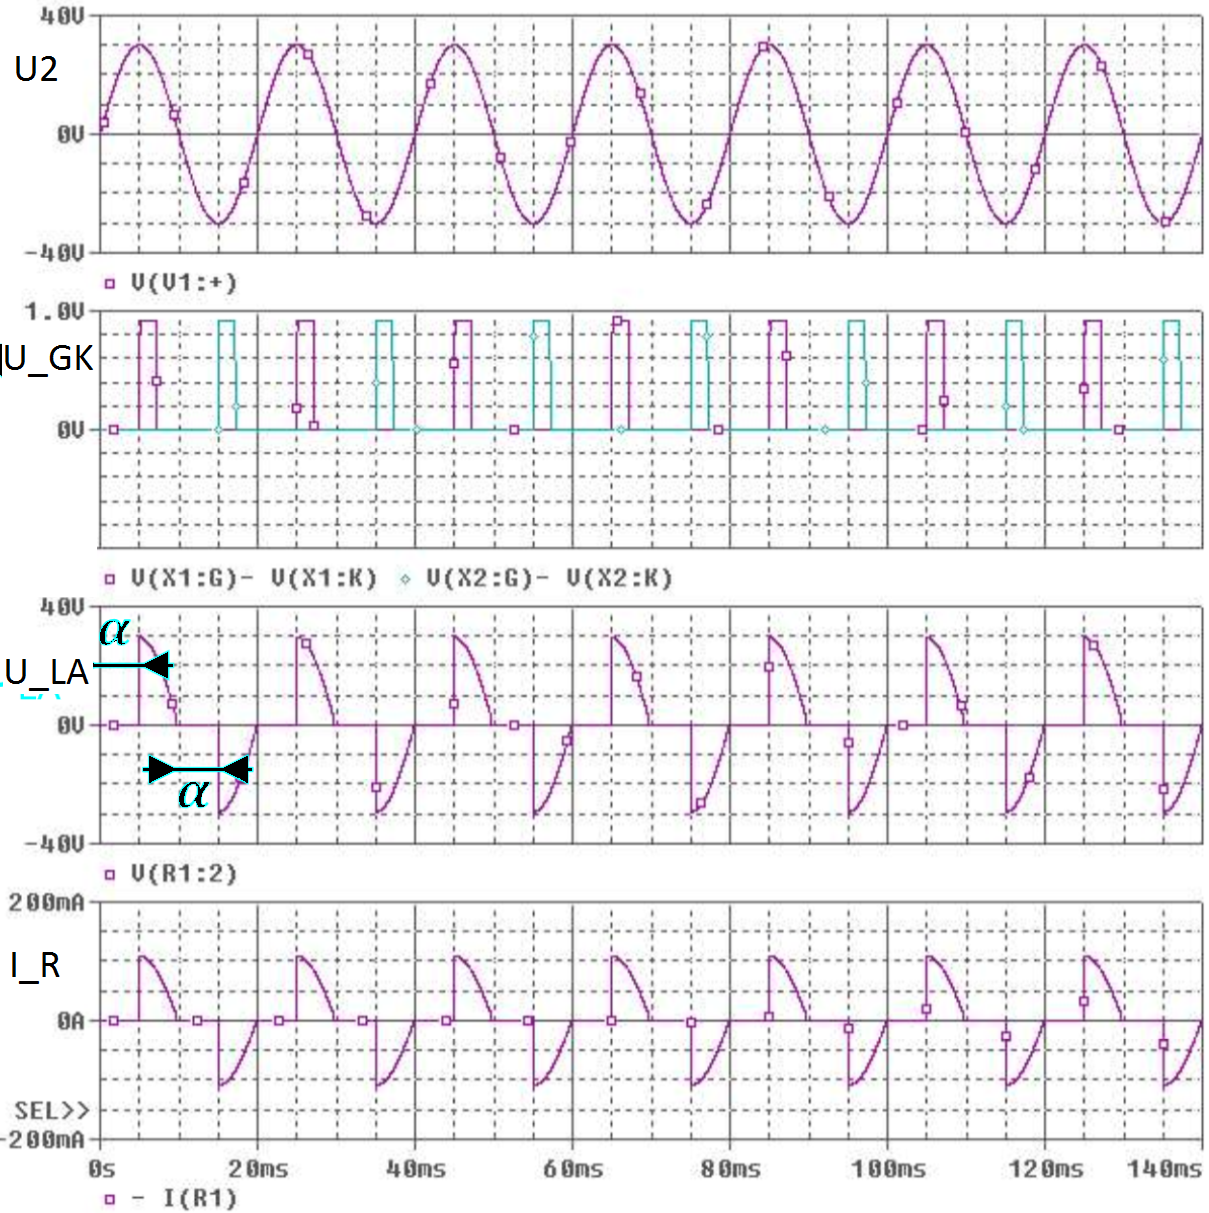
\includegraphics[width=\linewidth]{images/KLWSSteller}
\end{minipage}
\begin{minipage}{0.3\linewidth}
    \textbf{Lasttyp: R + L}\newline
    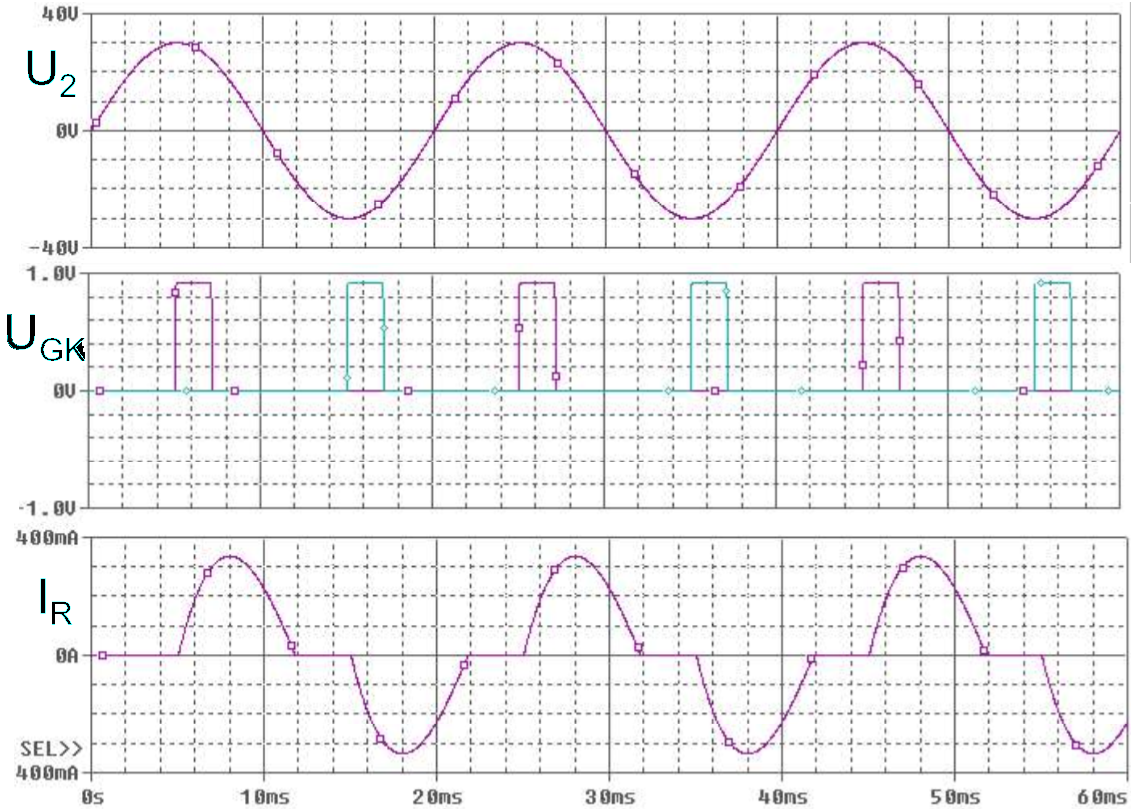
\includegraphics[width=\linewidth]{images/KLWSSteller2}
\end{minipage}


\subsubsection{Rechnungsbsp}
\textbf{Übung 4 Wechselstrom-Steller mit ohmischer Last}
\begin{longtable}{ p{.2\textwidth}  p{.50\textwidth}  p{.25\textwidth} |} %TODO Formeln einfügen
    Mittelwert&
    $ {U}_{R\; RAV} = \dfrac{1}{2\pi} \int\limits_{\alpha}^{\pi}U_{2m}\cdot sin(\beta) \diff \beta + \dfrac{1}{2\pi} \int\limits_{\pi +\alpha}^{2\pi}U_{2m}\cdot sin(\beta) \textbf{= 0} $ &
    $ \beta = \omega t $
    \\ 
    
    Effektivwert&
    $ U_{R\; RMS}= \sqrt{\frac{U_{2m}^2}{2\pi}\left( \int\limits_{\alpha}^{\pi} sin(\beta)^2 \diff \beta + \int\limits_{\pi +\alpha}^{2\pi} sin(\beta)^2 \diff \beta \right)} \newline
    \hspace*{1cm} =\sqrt{\frac{U_{2m}^2}{\pi}\int\limits_{\alpha}^{\pi} sin(\beta)^2 \diff\beta}
    = U_{2m}\sqrt{\frac{\pi - \alpha}{2 \pi}+ \frac{sin(2\alpha)}{4\pi}} = \frac{U_{2m}}{\sqrt{2}} $ &
    \\
    
    Wirkleistung&
    $ P = \frac{1}{2\pi}\int\limits_{0}^{2\pi} u_{R}(\beta)\cdot i_2(\beta)\cdot \diff \beta = \frac{U_{R\;RMS}^2}{R} \newline
     \hspace*{1cm} = \frac{U_{2m}^2}{2\pi R}\left(\pi - \alpha + sin(\alpha) \cdot cos(\alpha)\right)$& 
    \\
    
\end{longtable}

%\begin{minipage}{0.3\linewidth}
%    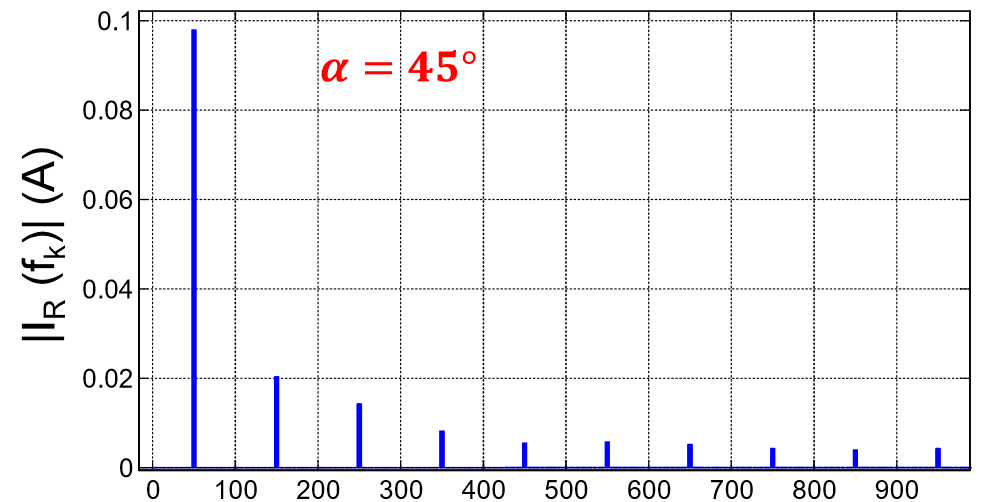
\includegraphics[width=\linewidth]{images/OW45WSSteller}
%    
%    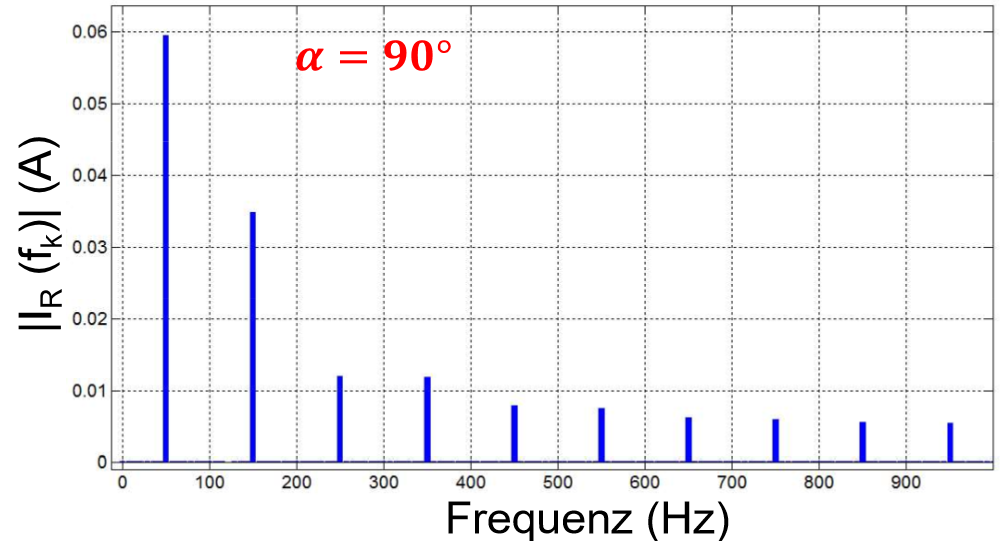
\includegraphics[width=\linewidth]{images/OW90WSSteller}
%\end{minipage}
\clearpage